\chapter{Analysis}\label{chap:analysis}


\tikz \draw[-latex,ultra thick]  node[right,fill=yellow,append after command={(a.south west) -- ($(a.south west)!0.4!(a.south east)$)},label={[inner sep=0]south east:$100$},
label={[inner sep=0]south west:$0$}] (a) {Current status: 40\% Converting the article to thesis format};
\vspace{1cm}


This chapter would be simply a copy of the Transactions on Robotics Vol.28(6) 2012 paper and 
more info on IQC multipliers (Zames-Falb etc.) missing from the article. Expected time for finishing:
 2 weeks (hopefully synced with Cesar's arrival).


\section{Quadratic Forms for Stability Analysis}
In the sequel, instead of 2-port networks, we rather consider system interconnections as 
depicted in \Cref{fig:uncic}. In this setting, $G$ is the model of the nominal bilateral 
teleoperation system and $\Delta$ is a block diagonal collection of uncertainties, such as 
the human, the environment, delays, etc. Stability tests are based on structural hypotheses 
on the diagonal blocks of the operator $\Delta$ such as gain bounds or passivity. These 
properties should allow us to develop numerically verifiable conditions for the system $G$ that 
guarantee interconnection stability. This is intuitive because we have no access to the actual 
$\Delta$ and we can only describe its components by means of indirect properties. Over the 
past three decades many classical stability results have been unified and generalized in 
this direction by utilizing quadratic forms (see \cite{megretski} and \cite{safonov,carsten2,iwasaki}).


\begin{figure}
\begin{subfigure}[b]{.5\linewidth}
\centering%
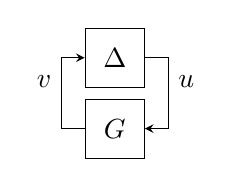
\begin{tikzpicture}[>=stealth,scale=0.6]
\node[draw,minimum size=0.75cm] (plant) at (0,0) {$G$};
\node[draw,minimum size=0.75cm] (unc) at (0,1.5) {$\Delta$};
\draw[->] (plant.west) -| ++(-5mm,10mm) node[left] {$v$} |- (unc.west);
\draw[->] (unc.east)   -| ++(5mm,-5mm) node[right] {$u$} |- (plant.east);
\end{tikzpicture}	
\caption{}\label{fig:uncic}
\end{subfigure}%
\begin{subfigure}[b]{.5\linewidth}
\centering%
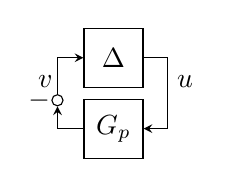
\begin{tikzpicture}[>=stealth,scale=0.6]
\node[draw,rectangle, minimum size=0.75cm] (plant) at (0,0) {$G_p$};
\node[draw,rectangle, minimum size=0.75cm] (unc) at (0,1.5cm) {$\Delta$};
\node[draw,circle,inner sep=0.5mm,label={[inner sep=0.1mm]180:$-$},label={[inner sep=0,yshift=1mm]135:$v$}] at ([shift={(-0.55cm,0.6cm)}]plant.west)(junc) {};
\draw[->] (plant.west) -| (junc.south);
\draw[->] (junc.north) |- (unc.west);
\draw[->] (unc.east) -| ++(0.5cm,-0.5cm) node[right]{$u$}|- (plant.east);
\end{tikzpicture}
\caption{}\label{fig:uncicpas}
\end{subfigure}
\caption{The general interconnection (a) and the assumed interconnection for passive systems (b). In general, the power variables require a sign change relative to the ``from" and ``to" ports in order to indicate the travel direction which translates to a negative sign in the block diagrams.}\label{fig:2}
\end{figure}

It is beyond the scope of this paper to include a comprehensive treatment of the subject, but for the 
sake of completeness, we present the general methodology by sampling a few important special cases. 
To begin with, consider the following reformulation of the conditions of the small-gain theorem:
\begin{equation}
\begin{aligned}
\|\Delta\|_\infty &\leq 1\\
\|G\|_\infty &< 1
\end{aligned} \iff
{\scriptstyle \begin{aligned}
\pmatr{\Delta(\iw)\\1}^*\pmatr{-1 &0\\0 &1}\pmatr{\Delta(\iw)\\1} &\geq 0\\
\pmatr{1\\G(\iw)}^*\pmatr{-1 &0\\0 &1}\pmatr{1\\G(\iw)} &< 0
\end{aligned}}
\label{eq:smqf}
\end{equation}
for all $\omega\in\Realext$. The middle {$2\times2$ matrix} on the right-hand side is called the 
``\emph{multiplier}'' (typically denoted by $\Pi$). It has been observed that the appearance of the 
same multiplier on both inequalities is far from a mere coincidence. In fact, it led to the following 
stability test: Assume that $G,\Delta\in \mathcal{RH}^{\bullet \times \bullet}_\infty$. Then, the 
$G-\Delta$ interconnection {in \Cref{fig:uncic}} is well posed and stable if there exists a 
Hermitian matrix $\Pi$ such that
\begin{equation}
\pmatr{\Delta(\iw)\\I}^*\!\!\!\Pi\pmatr{\Delta(\iw)\\I} \succeq 0,\
\pmatr{I\\G(\iw)}^*\!\!\!\Pi\pmatr{I\\G(\iw)} \prec 0  \label{eq:qcdelta}
\end{equation}
hold for all $\omega\in\Realext$; one only requires the mild technical hypothesis that the left-upper/right-lower 
block of $\Pi$ is negative/positive semi-definite. Thus, the intuition that we touched upon above is mathematically 
formalized by \eqref{eq:qcdelta}. Indeed, one can see that the former condition constrains the family of uncertainties,
 while the latter {provides the related condition} imposed on the plant for interconnection stability, both expressed 
in terms of the multiplier $\Pi$. In particular, we recover the passivity theorem in a similar fashion, if {using} 
the constant symmetric matrix $\Pi=\left(\begin{smallmatrix}0 &I \\ I &0 \end{smallmatrix} \right)$ as the multiplier 
under negative feedback. See \cite{safonov} for a lucid ``topological seperation" argument. For our example, assume that
\eqref{eq:qcdelta} holds for both inequalities for all $\omega$. Then, using the relations, $w=\Delta v,v=G w$ for all 
$u,y\in\LL_2$ we obtain the following contradiction
\begin{align}
0 &\preceq v^*\pmatr{\Delta\\I}^*\!\!\!\Pi\pmatr{\Delta\\I}v\\ &=\phantom{v^*}\pmatr{w\\v}^*\Pi\pmatr{w\\v}\\
&=w^*\pmatr{I\\G}^*\!\!\!\Pi\pmatr{I\\G}w \\&\prec 0, 
\end{align}
hence
\[
\operatorname{im}\pmatr{I\\G} \cap \operatorname{im}\pmatr{\Delta \\ I} =\{0\} ,\ \forall \omega\in\Realext.
\]
Using this we can conclude that 
\[
\det\pmatr{I &\Delta\\G &I}\neq 0\ \forall \omega\in\Realext
\]
Various other classical stability tests fall under this particular {scenario based on the so-called static 
(frequency-independent) multipliers which, therefore, presents} a significantly unified methodology.

If $\Delta$ admits a diagonal structure [as in \Cref{fig:portrep}], it is well known that the small-gain theorem 
and passivity theorem are conservative. A natural generalization toward a tighter analysis test is using a frequency-dependent 
$\Pi$ matrix, {which can be interpreted as} adding dynamics to the multiplier. Two prominent examples of 
interest are the celebrated upper bound computations for $\mu$ or $\kappa_m$ in robust control theory and, as we will 
show later, Llewellyn's stability conditions. As a shortcoming, these results are only valid for LTI operators but the 
real power and flexibility of these multiplier methods come from {their} generalizations to classes of nonlinear/time-varying 
operators via the IQC framework that appeared in \cite{megretski}.

An IQC for the input and output signals of $\Delta$ is expressed as
\begin{equation}{\displaystyle\infint{\pmatr{\widehat{\Delta(v)}(\iw)\\\hat{v}(\iw)}^*\Pi(\iw)\pmatr{\widehat{\Delta(v)}(\iw)\\\hat{v}(\iw)}d\omega}} \geq 0.
\label{eq:IQC}
\end{equation}
A bounded operator $\Delta:\mathcal{L}^m_2\to\mathcal{L}^n_2$ is said to satisfy the constraint defined by $\Pi(\iw)$ if \eqref{eq:IQC} holds for all $v\in\mathcal{L}^m_2$.
The following sufficient {stability condition for the interconnection in \Cref{fig:uncic}} forms the basis for the IQC framework.
\begin{thm}[\cite{megretski}] Let $G\in\mathcal{RH}^{n\times m}_\infty$ be given and let $\Delta:\mathcal{L}^m_2\to\mathcal{L}^n_2$ be a bounded causal operator. Suppose that
\begin{enumerate}
	\item for every $\tau\in[0,1]$, the interconnection of $G$ and $\tau\Delta$ is well posed;
	\item for every $\tau\in[0,1]$, $\tau\Delta$ satisfies the IQC defined by $\Pi(\iw)$ {which is bounded as a function of $\omega\in\Real$;}
	\item there exists some $\epsilon>0$ such that
	\begin{equation}
	\pmatr{I\\G(\iw)}^*\Pi(\iw)\pmatr{I\\G(\iw)} \preceq -\epsilon I\text{\ for all\ }\omega\in\mathbb{\Real}.
	\label{eq:IQCthmFDI}
	\end{equation}
\label{IQCthm}
\end{enumerate}
Then the $G-\Delta$ interconnection {in \Cref{fig:uncic}}  is stable.
\end{thm}
\begin{rem}\label{remiqc}
\begin{enumerate}
  \item Note that both properties 1 and 2 in \Cref{IQCthm} have to hold for $\tau\Delta$ 
if $\tau$ moves from $\tau=0$ (for which stability is obvious) to the target value $\tau=1$ 
(for which stability is desired). In our examples the left-upper $m\times m$ block (the right-lower 
$n\times n$ block) of $\Pi(\iw)$ is negative(positive) semi-definite for all $\omega\in\Realext$ 
respectively. It is then easy to see that \eqref{eq:IQC} implies property 2 in \Cref{IQCthm}; 
hence one only needs to verify \eqref{eq:IQC} for the original uncertainty $\Delta$.
\item
Often $\Pi(\iw)$ is a continuous function of $\omega\in\Realext$. Then property 3 is equivalent to
\begin{equation}
\pmatr{I\\G(\iw)}^*\Pi(\iw)\pmatr{I\\G(\iw)} \prec 0
\text{\ \ for all\ \ }\omega\in\Realext.
\label{eq:IQCthmFDI2}
\end{equation}
If $\Delta$ is LTI then \eqref{eq:IQC} holds for all $v\in\mathcal{L}^m_2$ if and only if
\begin{equation}
\pmatr{\Delta(\iw)\\I}^*\Pi(\iw)\pmatr{\Delta(\iw)\\I} \succeq 0
\text{\ \ for all\ \ }\omega\in\Real.
\label{fdidelta}
\end{equation}
The IQC reduces to a frequency-domain inequality (FDI). This provides the link to our introductory discussion.

Suppose that $\Delta$ is LTI and $\Pi(\iw)$ is a continuous function
of $\omega\in\Realext$. As we have illustrated above, \eqref{eq:IQCthmFDI2} and \eqref{fdidelta} imply
\begin{equation}
\det(I-G(\iw)\Delta(\iw))\neq 0\text{\ \ for all\ \ }\omega\in\Realext,
\end{equation}
which is the precise condition that forms the basis of SSV theory \cite{packdoyle}. This gives some intuition for the validity
of the IQC theorem and relates to $\mu$ in SSV theory. 
\item  In combination with the previous remarks, properties 2 and 3 imply
$\det(I-\tau G(\infty)\Delta(\infty))\neq 0$ for $\tau\in[0,1]$
which is nothing but property 1.
Two conclusions can be drawn: On one hand, under these circumstances property 1 is redundant in \Cref{IQCthm}. On the other 
hand, if 1 and 2 have been verified, it suffices to check \eqref{eq:IQCthmFDI2} only for finite $\omega\in\Real$ in order to infer stability with the IQC theorem.
\end{enumerate}
\end{rem}


If we have an IQC constraint that is satisfied for all $\Delta\in\bm{\Delta}$ with some particular uncertainty 
set $\bm{\Delta}$, checking robust stability boils down to the verification of the corresponding FDI \eqref{eq:IQCthmFDI} 
or \eqref{eq:IQCthmFDI2}. Instead of validating these in a frequency-by-frequency fashion, one can make use of 
the Kalman-Yakubovich-Popov (KYP) Lemma (see \cite{rantzerkyp} and below) in order to convert the FDI into 
a genuine linear matrix inequality (LMI) by using state space representations. For the finite frequency intervals, 
one can further use the Generalized KYP Lemma (\cite{genelKYP}) to limit the analysis to some physically relevant frequency band.

\section{Basic IQC Multiplier Classes}
In the previous section, we have shown how classical frequency domain techniques can be embedded into the IQC formulation. In this section, we focus on the types of existing multipliers for different uncertainty classes. Although they frequently appear in the robust control literature, we include them for completeness.


\subsection{Parametrized Passivity}\label{sec:osppass}
Another well-known version of the passivity theorem, {which we will denote as} theorem of parameterized passivity (see e.g. \cite[Thm. VI.5.10]{desvid}), allows to consider cases in which the ''non-passivity'' of some block is compensated by an excess of passivity in other blocks without endangering stability. This can even be utilized to determine the lowest tolerable level of passivity of the uncertainties for which a given interconnection remains stable. For output strictly passive uncertainties, stability can be characterized as in the next result, which is a direct consequence of the general IQC theorem.

\begin{coroll}\label{thm:desvidpass} {The interconnection of $G_p,\Delta\in \mathcal{RH}^{\bullet \times \bullet}_\infty$ as in \Cref{fig:uncicpas} is stable}
if there exist a ${p\geq 0}$ such that
\begin{align}
\pmatr{\Delta(\iw)\\I}^*\pmatr{-pI &I\\I &0}\pmatr{\Delta(\iw)\\ I} &\succeq 0 \label{eq:parampas1}\\
\pmatr{I\\ -G_p(\iw)}^*\pmatr{-pI &I\\I &0}\pmatr{I\\ -G_p(\iw)} &\prec 0 \label{eq:parampas2}
\end{align} hold for all $\omega\in\Realext$.
\end{coroll}

\begin{rem}Note that \eqref{eq:parampas1} and \eqref{eq:parampas2} are nothing but
\begin{align}
	\Delta(\iw) + \Delta^*(\iw) &\succeq p\Delta^*(\iw)\Delta(\iw),\label{parpas1}\\
	G_p(\iw) + G_p^*(\iw) &\succ -pI.\label{parpas2}
\end{align}
The case $p=0$ recovers the classical passivity theorem. Moreover, the larger the value of $p>0$, the smaller is the set of uncertainties described by \eqref{parpas1}, as illustrated in \Cref{fig:pregions} for different values of $p$. In fact, this result is used in Colgate's condition thanks to the damping term $b$ and closely related to the impedance bounds of Bounded Impedance Absolute Stability \cite{haddadizaad} using ``impedance circles".
%I did not understand the next sentence.
%After introducing dynamics to the multiplier, it is straightforward to utilize the test for the class of uncertainties that satisfy the conditions above.
\end{rem}

\begin{figure}%
\centering
\begin{tikzpicture}[>=stealth,scale=0.535]
\draw[<->] (-3,0) -- (3,0) node[right] {$Re$};
\draw[<->] (0,-3) -- (0,3) node[left] {$Im$};
\clip (-3,-3) rectangle (3,3);
\draw[pattern = checkerboard,opacity=0.5,color=black!10] (0,-3.5) rectangle (3,3);
\foreach \x in {10,3,2,1}{ \draw (\x,0) circle (\x);}
\draw[thick,->] (0.1,-2.5) -- (1.5,-1.5) node[right] {$p$};
\end{tikzpicture}
\caption{As $p$ increases, the admissible region for the Nyquist curves of $\Delta$ shrinks to smaller disks in the right half plane.}
\label{fig:pregions}%
\end{figure}


\subsection{Real Parametric Uncertainties}\label{sec:ltvenv}
In many applications, the uncertainties originate from the lack of the precision
on the actual values of the parameters in the system model. This applies in
particular to the models used in bilateral teleoperation. Parameters such as the
stiffness and the damping of the environment or the human arm are the simplest
examples of this kind. After re-scaling and shifting, the real parametric uncertainties
are assumed to take values in the interval $\left[ -r,r \right]$ centered around
the nominal value zero.

\subsubsection{LTI uncertain parameters} The well-known $DG$ multiplier family (\cite{meinsmafu,fantits}) is used to assess robustness against unknown but constant parameters. In fact, for all bounded functions $D:\mathbb{R}\mapsto(0,\infty)$ and $G:\mathbb{R}\mapsto i\mathbb{R}$ one has
\begin{equation*}
\pmatr{\delta\\1}^*\pmatr{-D(\omega) &G(\omega)\\G^*(\omega) &r^2D(\omega)}\pmatr{\delta\\1}\geq 0
%\label{eq:DGscalingderiv}
\end{equation*}
for all $\delta\in[-r,r]$, just because it reads as
$-D(\omega)|\delta|^2 + r^2 D(\omega) + (G(\omega)^*+G(\omega))\delta\geq 0$;
this holds since $|\delta|^2\leq r^2$, $D(\omega)>0$ and $G(\omega)+G(\omega)^*=0$.


\subsubsection{Time-varying parameters with arbitrary rate of variation}
In this case we employ constant multipliers; the time-varying parameter $\delta:[0,\infty)\mapsto [-r,r]$ satisfies the quadratic constraint
\begin{equation*}
\pmatr{\delta(t)\\1}^*\pmatr{-D &iG\\-iG &r^2D}\pmatr{\delta(t)\\1}\geq 0
%\label{eq:DGscalingderiv_arbfast}
\end{equation*}
for all $D>0$, $G\in\mathbb{R}$ and for all $t\geq 0$. This implies the validity of \eqref{eq:IQC} for the multiplication operator which
maps $v\in \mathcal{L}_2^n$ into $w\in\mathcal{L}_2^n$ with $w(t)=\delta(t)v(t)$.


\subsubsection{Time-varying parameters with bounded rate of variation} If there is a known bound on the rate-of-variation (ROV) of the time-varying parameter, it is conservative to use constant $DG$ scalings. To characterize slowly-varying real parametric uncertainties, we use the so-called ``swapping lemma" (\cite{helmersson,jonsson,koroglu}, cf. \cite{packardteng}) which allows to take the ROV bound explicitly into account. For the sake of completeness, we include a scalar version of this well known result from adaptive control.

\begin{lem}[Swapping Lemma]\label{lem:swap}
Consider the bounded and differentiable function $\delta:[0,\infty)\to\Real$ whose derivative is bounded as $|\dot{\delta}(t)| \leq d$ for all $t\geq 0$. Moreover, let $T(s) = C(sI-A)^{-1}B+D$ be a transfer function with a stable state-space realization and define
\begin{equation*}
T_c(s) :=  C(sI-A)^{-1}, \quad T_b(s) :=  (sI-A)^{-1}B.
%\label{eq:swapfunc}
\end{equation*}
If viewing $T$, $T_c$, $T_b$ and $\delta$ (by point-wise multiplication) as operators
$\mathcal{L}_2\to \mathcal{L}_2$, one has $\delta T = T\delta  + T_c \dot{\delta} T_b $ and thus
\begin{equation*}
\underbrace{\pmatr{T &T_c\\0 &I}}_{T_{\mathrm{left}}}\underbrace{
\pmatr{\delta\\ \dot{\delta}T_b}}_{\Delta_s} = \underbrace{\pmatr{\delta &0\\0 & \dot{\delta}I}}_{\Delta_x} \underbrace{\pmatr{T\\T_b}}_{T_{\mathrm{right}}}
%\label{eq:swapmeq}
\end{equation*}
where $x$, $s$ stand for ``eXtended'' and ``Stacked" respectively.
\end{lem}
We now claim that
\[
\Pi(\iw) = \pmatr{\star}^*{M}_s\pmatr{T_{\mathrm{left}}(\iw) &0\\0 &T_{\mathrm{right}}(\iw)}
\]
with
\[
{M}_s = \pmatr{-D_a &0 &iG_a &0\\0 &-D_b&0&iG_b\\ -iG_a &0 &r^2D_a &0\\0 &-iG_b &0 &d^2D_b}
\]
for $T^*D_aT > 0$, $D_b>0$ and $G_a$, $G_b\in\mathbb{R}$ is a valid IQC multiplier for the uncertainty $\Delta_s$. In fact,
one easily verifies
\[
\pmatr{\Delta_x(t)\\I}^TM_s\pmatr{\Delta_x(t)\\I} \succeq 0
\text{\ \ for all\ \ }t\geq 0
\]
in the time domain. If we choose any $v\in \LL_2$ and define
$w=\pmatr{\Delta_x\\I}T_{right}v,$
we hence infer $\int_0^\infty w(t)^TM_sw(t)\,dt\geq 0$. On the other hand, due to \Cref{lem:swap}, we also have
$$
w=\pmatr{T_{\mathrm{left}}\Delta_s\\T_{\mathrm{right}}}v=\pmatr{T_{\mathrm{left}} &0\\0 &T_{\mathrm{right}}}
\pmatr{\delta \\\dot{\delta}T_b\\1}
$$
which proves the claim. Thus, after augmenting the corresponding channel with zero columns so as to make the plant compatible with $\Delta_s$, the robustness test can be performed.


\subsection{Delay Uncertainty}\label{sec:delayiqc}

The delay robustness problem has been studied extensively and the dominating approach 
is the use of scattering transformations/wave variable techniques, among other methods 
(\cite{leungfa, eusebi, andersonspong, nieslotine, nieslotine2, hokayemspong, yokokohji, 
lozano, arcara, parkcho, aziminejad, leespong}). We refer to the survey article \cite{hokayemspong} 
for a detailed exposition of these methods. A great deal of research has been devoted to 
delay robustness tests in robust control that are applicable to a wide class of teleoperation 
systems. We also refer to \cite{richard} for a general treatment of the subject (e.g. based on 
Lyapunov-Krasovskii functionals) and to IQC based results as e.g. in \cite{scorletti,junsafonov,
kaorantzer,niculescu}.

Here, we consider constant but uncertain delays and the maximum delay duration is bounded 
from above by $\bar{\tau} > 0$ seconds. We emphasize that it requires only a simple 
modification of the multiplier in order to arrive at robustness tests for different types 
of delays as reported in the literature.


If using the uncertainty $\Delta(s)=e^{-s\tau}$ in the configuration of \Cref{fig:uncic}, 
the nominal value $\tau=0$ leads to $\Delta(s)=1$ and not to zero as desired. This is resolved 
by utilizing the shifted uncertainty $\tilde{\Delta}(s)=e^{-s\tau}-1$ and correspondingly 
modifying the system to $\tilde{G}$ (by unity feedback around $G$) as in 
\Cref{fig:uncicpasdelay2} and without modifying the interconnection (cf. \cite{leungfa}).

\begin{figure}
\begin{subfigure}[b]{.4\linewidth}
\centering%
\begin{tikzpicture}[>=stealth,scale=0.8,transform shape]
\draw[loosely dashed,fill=black!5] (-1.4,-0.7) rectangle (1.3,1.1);
\draw[loosely dashed,fill=black!5] (-1.4,1.4) rectangle (1.3,3.2);
\node[draw,inner sep=1mm,minimum height=1cm] (delay) at (0,2.5) {$e^{-s\tau}$};
\node[draw,inner sep=3.5mm] (plant) at (0,0) {$G$};
\path (delay.east) -| ++(0.5,-0.7) node[draw,fill=white,circle,inner sep=2pt,label={[inner sep=0mm]above right:\tiny$+$},label={[inner sep=0mm]below left:\tiny$-$}] (junc1) {} --%
++(0,-1) node[draw,fill=white,circle,inner sep=2pt,label={[inner sep=0mm]above right:\tiny$+$},label={[inner sep=0mm]below left:\tiny$+$}] (junc2) {}%
 |- (plant.east);
\draw[->] (plant.west) -| ++(-0.5,1) |- (delay.west);
\draw[->] (delay.east) -| (junc1.north);
\draw[->] (junc1.south) -- (junc2.north);
\draw[->] (junc2.south) |- (plant.east);
\draw[<-] (junc2.west) -- ++(-1.9,0);
\draw[<-] (junc1.west) -- ++(-1.9,0);
\node[above left=2mm and 3.0mm of delay.west] (tildelay) {$\tilde{\Delta}$};
\node[below left=2mm and 3mm of plant.west] (tilplant) {$\tilde{G}$};
\end{tikzpicture}
\phantomsubcaption\label{fig:uncicpasdelay2}%
\end{subfigure}%
\begin{subfigure}[b]{.6\linewidth}
\centering%
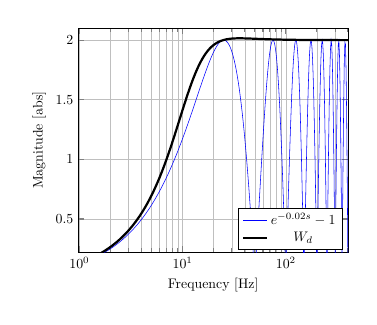
\begin{tikzpicture}[scale=0.5]
\begin{semilogxaxis}[%
legend style={at={(0.98,0.2)}},
no markers,
grid=both,
domain=1:400,
ymin=0.220,
ymax=2.1,
xmax=400,
samples=450,
tick style={thick},
xlabel=Frequency {[Hz]},
ylabel=Magnitude {[abs]}]
\addplot{sqrt(((-1+cos(0.02*deg(2*pi*x)))^2 + (sin(0.02*deg(2*pi*x)))^2)};
\addplot[ultra thick]{sqrt(((1600*pi^2*x^2 + 1)*(10000*pi^2*x^2 + 10387729))/(2500*(1600*pi^4*x^4 + 1028164*pi^2*x^2 + 3805656100))};
\legend{$e^{-0.02s}-1$,$W_d$}
\end{semilogxaxis}
\end{tikzpicture}
\phantomsubcaption\label{fig:delayvsW}%
\end{subfigure}
\caption{(a) Rewriting the interconnection such that $\tau=0$ implies $\tilde{\Delta}=0$. (b) Frequency domain covering of the shifted delay operator.}\label{fig:3}
\end{figure}

The uncertainty is then characterized by using two properties of $\tilde \Delta$: For all $\omega,\tau$, the complex number $z=e^{-\iw{\tau}}-1$ is located on the unit circle centered at $(-1,0)$ in the complex plane. Since condition $\abs{z+1}=1$ translates into $z^*z+z^*+z=0$, we infer
for all bounded $\Omega:\Real\to\Real$ that
\begin{equation}
\pmatr{\tilde{\Delta}(\iw)\\1}^*\pmatr{\Omega(\omega) &\Omega(\omega)\\ \Omega(\omega) &0}\pmatr{\tilde{\Delta}(\iw)\\1} = 0\ \ \forall\omega\in\Real
\label{eq:onthecircle}
\end{equation}
for any delay time $\tau\in\Real$. Furthermore, we need to take the low frequency property of the magnitude of the frequency response into account. This is typically captured by a frequency dependent weight. If we define,
\begin{equation*}
W_d(s)= 2\frac{(s+ \frac{4}{\pi\bar{\tau}}) (s+ \frac{\beta}{\bar{\tau}})}{(s-\frac{\pi}{2\bar{\tau}}e^{i\theta})(s-\frac{\pi}{2\bar{\tau}}e^{-i\theta})}
%\label{eq:delayweightformula}
\end{equation*}
with $\theta=\left( \frac{\pi}{2}\right)^2$ and some small $\beta>0$, then $W_d$ covers the delay uncertainty in the sense that $|\tilde{\Delta}(\iw)|\leq |W(\iw)|$ for all $\omega\in\Real$ and for all $\tau\in [0,\bar{\tau}]$. An example of magnitude covering is shown in \Cref{fig:delayvsW}.

This property, in turn, translates into $(\tilde{\Delta})^*\tilde{\Delta}\leq (W_d)^*W_d$ for all $\omega\in\Real$. Then we can utilize the classical $D$-scalings to obtain the following constraint with a dynamic multiplier:
\begin{equation}
\pmatr{\star}^*\pmatr{-\mathcal{D}(\omega) &0\\0 &W_d(\iw)^*\mathcal{D}(\omega)W_d(\iw)}\pmatr{\tilde{\Delta}(\iw)\\1} \geq 0
\label{eq:normbounded}
\end{equation}
for all bounded $\mathcal{D}:\Real\to (0,\infty)$. Then the overall multiplier family results from a  conic combination of \eqref{eq:onthecircle} and \eqref{eq:normbounded}:
\[
%\arraycolsep.3ex
\pmatr{\star}^*\pmatr{-\mathcal{D}+\Omega &\Omega\\
\Omega &W_d^*\mathcal{D}W_d}\pmatr{\tilde{\Delta}\\1}
\geq 0 \quad \forall\omega\in\Real_e
\]